
%% bare_conf.tex
%% V1.3
%% 2007/01/11
%% by Michael Shell
%% See:
%% http://www.michaelshell.org/
%% for current contact information.
%%
%% This is a skeleton file demonstrating the use of IEEEtran.cls
%% (requires IEEEtran.cls version 1.7 or later) with an IEEE conference paper.
%%
%% Support sites:
%% http://www.michaelshell.org/tex/ieeetran/
%% http://www.ctan.org/tex-archive/macros/latex/contrib/IEEEtran/
%% and
%% http://www.ieee.org/

%%*************************************************************************
%% Legal Notice:
%% This code is offered as-is without any warranty either expressed or
%% implied; without even the implied warranty of MERCHANTABILITY or
%% FITNESS FOR A PARTICULAR PURPOSE! 
%% User assumes all risk.
%% In no event shall IEEE or any contributor to this code be liable for
%% any damages or losses, including, but not limited to, incidental,
%% consequential, or any other damages, resulting from the use or misuse
%% of any information contained here.
%%
%% All comments are the opinions of their respective authors and are not
%% necessarily endorsed by the IEEE.
%%
%% This work is distributed under the LaTeX Project Public License (LPPL)
%% ( http://www.latex-project.org/ ) version 1.3, and may be freely used,
%% distributed and modified. A copy of the LPPL, version 1.3, is included
%% in the base LaTeX documentation of all distributions of LaTeX released
%% 2003/12/01 or later.
%% Retain all contribution notices and credits.
%% ** Modified files should be clearly indicated as such, including  **
%% ** renaming them and changing author support contact information. **
%%
%% File list of work: IEEEtran.cls, IEEEtran_HOWTO.pdf, bare_adv.tex,
%%                    bare_conf.tex, bare_jrnl.tex, bare_jrnl_compsoc.tex
%%*************************************************************************

% *** Authors should verify (and, if needed, correct) their LaTeX system  ***
% *** with the testflow diagnostic prior to trusting their LaTeX platform ***
% *** with production work. IEEE's font choices can trigger bugs that do  ***
% *** not appear when using other class files.                            ***
% The testflow support page is at:
% http://www.michaelshell.org/tex/testflow/



% Note that the a4paper option is mainly intended so that authors in
% countries using A4 can easily print to A4 and see how their papers will
% look in print - the typesetting of the document will not typically be
% affected with changes in paper size (but the bottom and side margins will).
% Use the testflow package mentioned above to verify correct handling of
% both paper sizes by the user's LaTeX system.
%
% Also note that the "draftcls" or "draftclsnofoot", not "draft", option
% should be used if it is desired that the figures are to be displayed in
% draft mode.
%
\documentclass[conference]{IEEEtran}
% Add the compsoc option for Computer Society conferences.
%
% If IEEEtran.cls has not been installed into the LaTeX system files,
% manually specify the path to it like:
% \documentclass[conference]{../sty/IEEEtran}





% Some very useful LaTeX packages include:
% (uncomment the ones you want to load)


% *** MISC UTILITY PACKAGES ***
%
%\usepackage{ifpdf}
% Heiko Oberdiek's ifpdf.sty is very useful if you need conditional
% compilation based on whether the output is pdf or dvi.
% usage:
% \ifpdf
%   % pdf code
% \else
%   % dvi code
% \fi
% The latest version of ifpdf.sty can be obtained from:
% http://www.ctan.org/tex-archive/macros/latex/contrib/oberdiek/
% Also, note that IEEEtran.cls V1.7 and later provides a builtin
% \ifCLASSINFOpdf conditional that works the same way.
% When switching from latex to pdflatex and vice-versa, the compiler may
% have to be run twice to clear warning/error messages.

\usepackage{graphicx}
\usepackage{flushend}




% *** CITATION PACKAGES ***
%
\usepackage{cite}
% cite.sty was written by Donald Arseneau
% V1.6 and later of IEEEtran pre-defines the format of the cite.sty package
% \cite{} output to follow that of IEEE. Loading the cite package will
% result in citation numbers being automatically sorted and properly
% "compressed/ranged". e.g., [1], [9], [2], [7], [5], [6] without using
% cite.sty will become [1], [2], [5]--[7], [9] using cite.sty. cite.sty's
% \cite will automatically add leading space, if needed. Use cite.sty's
% noadjust option (cite.sty V3.8 and later) if you want to turn this off.
% cite.sty is already installed on most LaTeX systems. Be sure and use
% version 4.0 (2003-05-27) and later if using hyperref.sty. cite.sty does
% not currently provide for hyperlinked citations.
% The latest version can be obtained at:
% http://www.ctan.org/tex-archive/macros/latex/contrib/cite/
% The documentation is contained in the cite.sty file itself.






% *** GRAPHICS RELATED PACKAGES ***
%
\ifCLASSINFOpdf
  % \usepackage[pdftex]{graphicx}
  % declare the path(s) where your graphic files are
  % \graphicspath{{../pdf/}{../jpeg/}}
  % and their extensions so you won't have to specify these with
  % every instance of \includegraphics
  % \DeclareGraphicsExtensions{.pdf,.jpeg,.png}
\else
  % or other class option (dvipsone, dvipdf, if not using dvips). graphicx
  % will default to the driver specified in the system graphics.cfg if no
  % driver is specified.
  % \usepackage[dvips]{graphicx}
  % declare the path(s) where your graphic files are
  % \graphicspath{{../eps/}}
  % and their extensions so you won't have to specify these with
  % every instance of \includegraphics
  % \DeclareGraphicsExtensions{.eps}
\fi
% graphicx was written by David Carlisle and Sebastian Rahtz. It is
% required if you want graphics, photos, etc. graphicx.sty is already
% installed on most LaTeX systems. The latest version and documentation can
% be obtained at: 
% http://www.ctan.org/tex-archive/macros/latex/required/graphics/
% Another good source of documentation is "Using Imported Graphics in
% LaTeX2e" by Keith Reckdahl which can be found as epslatex.ps or
% epslatex.pdf at: http://www.ctan.org/tex-archive/info/
%
% latex, and pdflatex in dvi mode, support graphics in encapsulated
% postscript (.eps) format. pdflatex in pdf mode supports graphics
% in .pdf, .jpeg, .png and .mps (metapost) formats. Users should ensure
% that all non-photo figures use a vector format (.eps, .pdf, .mps) and
% not a bitmapped formats (.jpeg, .png). IEEE frowns on bitmapped formats
% which can result in "jaggedy"/blurry rendering of lines and letters as
% well as large increases in file sizes.
%
% You can find documentation about the pdfTeX application at:
% http://www.tug.org/applications/pdftex





% *** MATH PACKAGES ***
%
%\usepackage[cmex10]{amsmath}
% A popular package from the American Mathematical Society that provides
% many useful and powerful commands for dealing with mathematics. If using
% it, be sure to load this package with the cmex10 option to ensure that
% only type 1 fonts will utilized at all point sizes. Without this option,
% it is possible that some math symbols, particularly those within
% footnotes, will be rendered in bitmap form which will result in a
% document that can not be IEEE Xplore compliant!
%
% Also, note that the amsmath package sets \interdisplaylinepenalty to 10000
% thus preventing page breaks from occurring within multiline equations. Use:
%\interdisplaylinepenalty=2500
% after loading amsmath to restore such page breaks as IEEEtran.cls normally
% does. amsmath.sty is already installed on most LaTeX systems. The latest
% version and documentation can be obtained at:
% http://www.ctan.org/tex-archive/macros/latex/required/amslatex/math/





% *** SPECIALIZED LIST PACKAGES ***
%
%\usepackage{algorithmic}
% algorithmic.sty was written by Peter Williams and Rogerio Brito.
% This package provides an algorithmic environment fo describing algorithms.
% You can use the algorithmic environment in-text or within a figure
% environment to provide for a floating algorithm. Do NOT use the algorithm
% floating environment provided by algorithm.sty (by the same authors) or
% algorithm2e.sty (by Christophe Fiorio) as IEEE does not use dedicated
% algorithm float types and packages that provide these will not provide
% correct IEEE style captions. The latest version and documentation of
% algorithmic.sty can be obtained at:
% http://www.ctan.org/tex-archive/macros/latex/contrib/algorithms/
% There is also a support site at:
% http://algorithms.berlios.de/index.html
% Also of interest may be the (relatively newer and more customizable)
% algorithmicx.sty package by Szasz Janos:
% http://www.ctan.org/tex-archive/macros/latex/contrib/algorithmicx/




% *** ALIGNMENT PACKAGES ***
%
%\usepackage{array}
% Frank Mittelbach's and David Carlisle's array.sty patches and improves
% the standard LaTeX2e array and tabular environments to provide better
% appearance and additional user controls. As the default LaTeX2e table
% generation code is lacking to the point of almost being broken with
% respect to the quality of the end results, all users are strongly
% advised to use an enhanced (at the very least that provided by array.sty)
% set of table tools. array.sty is already installed on most systems. The
% latest version and documentation can be obtained at:
% http://www.ctan.org/tex-archive/macros/latex/required/tools/


%\usepackage{mdwmath}
%\usepackage{mdwtab}
% Also highly recommended is Mark Wooding's extremely powerful MDW tools,
% especially mdwmath.sty and mdwtab.sty which are used to format equations
% and tables, respectively. The MDWtools set is already installed on most
% LaTeX systems. The lastest version and documentation is available at:
% http://www.ctan.org/tex-archive/macros/latex/contrib/mdwtools/


% IEEEtran contains the IEEEeqnarray family of commands that can be used to
% generate multiline equations as well as matrices, tables, etc., of high
% quality.


%\usepackage{eqparbox}
% Also of notable interest is Scott Pakin's eqparbox package for creating
% (automatically sized) equal width boxes - aka "natural width parboxes".
% Available at:
% http://www.ctan.org/tex-archive/macros/latex/contrib/eqparbox/





% *** SUBFIGURE PACKAGES ***
%\usepackage[tight,footnotesize]{subfigure}
% subfigure.sty was written by Steven Douglas Cochran. This package makes it
% easy to put subfigures in your figures. e.g., "Figure 1a and 1b". For IEEE
% work, it is a good idea to load it with the tight package option to reduce
% the amount of white space around the subfigures. subfigure.sty is already
% installed on most LaTeX systems. The latest version and documentation can
% be obtained at:
% http://www.ctan.org/tex-archive/obsolete/macros/latex/contrib/subfigure/
% subfigure.sty has been superceeded by subfig.sty.



%\usepackage[caption=false]{caption}
%\usepackage[font=footnotesize]{subfig}
% subfig.sty, also written by Steven Douglas Cochran, is the modern
% replacement for subfigure.sty. However, subfig.sty requires and
% automatically loads Axel Sommerfeldt's caption.sty which will override
% IEEEtran.cls handling of captions and this will result in nonIEEE style
% figure/table captions. To prevent this problem, be sure and preload
% caption.sty with its "caption=false" package option. This is will preserve
% IEEEtran.cls handing of captions. Version 1.3 (2005/06/28) and later 
% (recommended due to many improvements over 1.2) of subfig.sty supports
% the caption=false option directly:
%\usepackage[caption=false,font=footnotesize]{subfig}
%
% The latest version and documentation can be obtained at:
% http://www.ctan.org/tex-archive/macros/latex/contrib/subfig/
% The latest version and documentation of caption.sty can be obtained at:
% http://www.ctan.org/tex-archive/macros/latex/contrib/caption/




% *** FLOAT PACKAGES ***
%
%\usepackage{fixltx2e}
% fixltx2e, the successor to the earlier fix2col.sty, was written by
% Frank Mittelbach and David Carlisle. This package corrects a few problems
% in the LaTeX2e kernel, the most notable of which is that in current
% LaTeX2e releases, the ordering of single and double column floats is not
% guaranteed to be preserved. Thus, an unpatched LaTeX2e can allow a
% single column figure to be placed prior to an earlier double column
% figure. The latest version and documentation can be found at:
% http://www.ctan.org/tex-archive/macros/latex/base/



%\usepackage{stfloats}
% stfloats.sty was written by Sigitas Tolusis. This package gives LaTeX2e
% the ability to do double column floats at the bottom of the page as well
% as the top. (e.g., "\begin{figure*}[!b]" is not normally possible in
% LaTeX2e). It also provides a command:
%\fnbelowfloat
% to enable the placement of footnotes below bottom floats (the standard
% LaTeX2e kernel puts them above bottom floats). This is an invasive package
% which rewrites many portions of the LaTeX2e float routines. It may not work
% with other packages that modify the LaTeX2e float routines. The latest
% version and documentation can be obtained at:
% http://www.ctan.org/tex-archive/macros/latex/contrib/sttools/
% Documentation is contained in the stfloats.sty comments as well as in the
% presfull.pdf file. Do not use the stfloats baselinefloat ability as IEEE
% does not allow \baselineskip to stretch. Authors submitting work to the
% IEEE should note that IEEE rarely uses double column equations and
% that authors should try to avoid such use. Do not be tempted to use the
% cuted.sty or midfloat.sty packages (also by Sigitas Tolusis) as IEEE does
% not format its papers in such ways.





% *** PDF, URL AND HYPERLINK PACKAGES ***
%
%\usepackage{url}
% url.sty was written by Donald Arseneau. It provides better support for
% handling and breaking URLs. url.sty is already installed on most LaTeX
% systems. The latest version can be obtained at:
% http://www.ctan.org/tex-archive/macros/latex/contrib/misc/
% Read the url.sty source comments for usage information. Basically,
% \url{my_url_here}.





% *** Do not adjust lengths that control margins, column widths, etc. ***
% *** Do not use packages that alter fonts (such as pslatex).         ***
% There should be no need to do such things with IEEEtran.cls V1.6 and later.
% (Unless specifically asked to do so by the journal or conference you plan
% to submit to, of course. )


% correct bad hyphenation here
\hyphenation{op-tical net-works semi-conduc-tor}
%\usepackage{float}
%\floatstyle{boxed}
%\restylefloat{figure}

\begin{document}
%
% paper title
% can use linebreaks \\ within to get better formatting as desired

\bibliographystyle{plain}

\title{Stencil Code Optimization for GPUs Through Machine Learning}


% author names and affiliations
% use a multiple column layout for up to three different
% affiliations
\author{\IEEEauthorblockN{Adam Barker}
\IEEEauthorblockA{%College of Engineering and Applied Science\\
University of Colorado at Colorado Springs\\
abarker2@uccs.edu}}

% conference papers do not typically use \thanks and this command
% is locked out in conference mode. If really needed, such as for
% the acknowledgment of grants, issue a \IEEEoverridecommandlockouts
% after \documentclass

% for over three affiliations, or if they all won't fit within the width
% of the page, use this alternative format:
% 
%\author{\IEEEauthorblockN{Michael Shell\IEEEauthorrefmark{1},
%Homer Simpson\IEEEauthorrefmark{2},
%James Kirk\IEEEauthorrefmark{3}, 
%Montgomery Scott\IEEEauthorrefmark{3} and
%Eldon Tyrell\IEEEauthorrefmark{4}}
%\IEEEauthorblockA{\IEEEauthorrefmark{1}School of Electrical and Computer Engineering\\
%Georgia Institute of Technology,
%Atlanta, Georgia 30332--0250\\ Email: see http://www.michaelshell.org/contact.html}
%\IEEEauthorblockA{\IEEEauthorrefmark{2}Twentieth Century Fox, Springfield, USA\\
%Email: homer@thesimpsons.com}
%\IEEEauthorblockA{\IEEEauthorrefmark{3}Starfleet Academy, San Francisco, California 96678-2391\\
%Telephone: (800) 555--1212, Fax: (888) 555--1212}
%\IEEEauthorblockA{\IEEEauthorrefmark{4}Tyrell Inc., 123 Replicant Street, Los Angeles, California 90210--4321}}




% use for special paper notices
%\IEEEspecialpapernotice{(Invited Paper)}




% make the title area
\maketitle


\begin{abstract}
%\boldmath
The microprocessor field today has begun to reach its limits as power and thermal constraints have been met and no longer can much leverage
of increasing the processor's clock speed be achieved. Thus, much of the scientific and engineering community has shifted to using many-core
architectures, such as GPUs, in order to do highly-parallel computations. Problems in this field have arisen however, as it becomes increasingly
more difficult for programmers to effectively optimize their code for the ever-changing architectures of GPUs today.
This paper will focus on the use of machine learning techniques in order to perform a combination of known optimizations on stencil codes for
NVIDIA's Compute Unified Device Architecture (CUDA) based GPUs and GPGPUs in order to automate optimizations of highly-parallel computations
for CUDA GPUs.

\end{abstract}
% IEEEtran.cls defaults to using nonbold math in the Abstract.
% This preserves the distinction between vectors and scalars. However,
% if the conference you are submitting to favors bold math in the abstract,
% then you can use LaTeX's standard command \boldmath at the very start
% of the abstract to achieve this. Many IEEE journals/conferences frown on
% math in the abstract anyway.

% no keywords




% For peer review papers, you can put extra information on the cover
% page as needed:
% \ifCLASSOPTIONpeerreview
% \begin{center} \bfseries EDICS Category: 3-BBND \end{center}
% \fi
%
% For peerreview papers, this IEEEtran command inserts a page break and
% creates the second title. It will be ignored for other modes.
\IEEEpeerreviewmaketitle



\section{Introduction}
% no \IEEEPARstart
Due to power and thermal constraints, the domain of micro-processors no longer benefits from increases in clock frequency\cite{Datta}.
This problem has shifted the focus of parallel computing to advanced many-core architectures, such as those present among GPUs.
However, this transition has led to problems in software development as programmers have difficulty in successfully optimizing
GPU kernels to efficiently use the resources provided by the architecture. This hampering occurs regardless of new programming models
such as CUDA and OpenCL as programmers have difficulty understanding the underlying architecture in order to correctly optimize kernels
for the GPU\cite{Zhang}. Also, NVIDIA typically updates its GPU architecture every one to two years, each with brand new layouts which
make programmers have to learn the new architecture in order to optimize code correctly.

Stencil computations are widely used in scientific computing on structured grids and in Partial Differential Equation (PDE) solvers for
domains such as computational fluid dynamics and other finite-difference computations\cite{Mici, Nguy, Jaeger, Datta, Gana, Zhang, NVIDIA}. Stencil computations use nearest-neighbor calculations
to approximate the value of the current node. In explicitly iterative stencil computations, a computationally-intensive kernel is used to
update all nodes in the grid at distinct time steps. Due to this, stencils benefit highly when placed on SIMT (Single Instruction Multiple Thread)
architectures, such as those on GPUs. However, due to the massive number of threads being run on a single grid, the number of memory accesses for
each time step is enormous and thus, stencil computations are generally memory-bound. These memory accesses typically contain overlap between threads
as each node shares neighbors with other nodes, so exploiting this property allows for optimizations that are crucial to leveraging data-level
parallelism inherent in these computations\cite{Zhang}.

\begin{figure}[h]
	\centering
		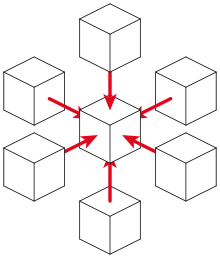
\includegraphics[width=5cm]{stencil-7.png}
		\caption{A 6-point Von-Neuman stencil (credit: wikipedia.org)}
\end{figure}

Auto-tuning of stencil kernels has become a fairly large area of study in order to work around the necessity of knowledge of the low-level specifications
of the architecture in order to optimize the kernel. However, these auto-tuners may have to look in a parameter space that is upwards of 40 million
combinations that may take months to fully check every single one for optimal performance\cite{Datta}. This then creates a demand for a faster optimization
process that is still automated in order to create a process that is viable for industry use. Thus, machine learning may be a good option for automatic
optimization as it can use reinforcement learning paired with statistical machine learning and genetic algorithms in order to explore the parameter space
much faster. Using machine learning may also overcome another downfall of auto-tuning in that each auto-tuner is generally programmed for one architecture,
 whereas a learner can learn architectures as well and correctly optimize for them.

This work will focus on optimizing stencil codes on NVIDIA GPUs. The list of GPUs being used to conduct this research consists of two consumer-level
GPUs (GTX 680, GTX 480) and one General-Purpose computing GPU (Tesla C2050). Between the cards, two architectures are tested: the GTX 480 and the Tesla
C2050 use the Fermi architecture, whereas the GTX 680 uses the latest Kepler architecture. It should also be noted that the Tesla C2050 is a GPGPU that
has more double-precision floating point processors than the GTX 680 and GTX 480, which may create differing results for optimizations on double-precision
kernels\cite{NVIDIA}. These architectures differ widely and should be able to show how the optimizations differ from chip to chip.

\section{Related Work}
Due to the high-memory bandwidth requirements needed for stencil computations, much of the research done for optimization focuses primarily on memory layout techniques and exploiting lower levels of memory such as cache and shared memory. One technique is 2.5D blocking in order to create the grid layout in memory by only finding the x and y values of the thread block and keeping the z axis constant\cite{Datta}. However, another paper has been written on a different blocking scheme that is optimal for stencil computations called 3.5D blocking which combines 3D blocking with 2.5D blocking in order to lower the amount of memory accesses for a stencil code\cite{Nguy}. Another promising research paper was done on efficient data layout for stencil codes on GPUs and similar multithreaded architectures which provides another key optimization to incorporate in this research\cite{Jaeger}. Other notable research has been done on exploiting memory re-usage in 3D finite-difference calcuatlions\cite{Mici} and may also be considered for inclusion in this research.  


As for current work in machine learning applications for stencil code optimization, a short study was done to see if statistical machine learning and genetic programming could be used to optimize stencil kernels on multicore architecture\cite{Gana}. However, no papers could be found on machine learning for stencil code optimization on GPUs, so this paper should serve as a basis step into researching feasable machine learning techniques to be used on optimizing stencil code for GPUs.


Also, many auto-tuning and auto-generation techniques have been explored, most notably research done on the auto-tuning of 3D stencil codes on GPU clusters, which details a rigorous auto-tuning and auto-generation framework for CUDA devices, which can be incorporated into our work by benchmarking our machine learning algorithm's speed against the speed of a similar auto-tuning mechanism based on the research\cite{Zhang}. 

\section{Motivation}
Due to the large number of optimizations to be considered, difficult architecture layouts to master, and constantly changing hardware, machine learning is a desirable approach to automatically optimizing stencil kernels quickly on any architecture. This would then allow for more advanced simulations to be done as they are no longer constrained by the difficulty to optimize stencil codes and programmers will no longer need to have a deep understanding of the underlying architecture in order to optimize stencil codes quickly and efficiently. This research will hopefully provide a framework to create a machine learning technique to optimize stencil kernels on advanced GPU and GPGPU architectures.

\section{Proposed Approach}
The research will focus on creating a set of configurable stencil kernels that allow inputs for grid dimensions, block dimensions, and shared memory size per block so that training data can be quickly and easily generated by generating stencil codes with randomly passed in parameters. This data will then be traversed by the machine learning algorithm and will predict what optimizations will be best for a given stencil kernel and data set based on this randomly generated training data. The timeline of this approach is as follows:
\begin{description}
   \item[Week 3] {Implement configurable stencil kernels in CUDA.}
   \item[Week 4] {Set up machine learning algorithm and begin testing/debugging.}
   \item[Week 5] {Test on training data, fine tune learner. Explore other machine learning possibilities.} 
   \item[Week 8] {Finalize learning algorithm and collect results on test data set. Write paper draft.}
   \item[Week 9] {Finalize paper for submission.}
\end{description}
The goal of this research is to create a machine learner that can optimize stencil kernels that are on par with those that are hand-optimized, but in a fraction of the time. The learner should be able to optimize for any given CUDA-based architecture 

\section{Experiments}
Four experimental data sets will be generated for the machine learning algorithm to use. These data sets will consist of a few thousand randomly-configured stencil codes which can be used by the machine learner in order for it to be able to select a set of optimizations to perform on the given kernel so that the kernel can be as optimized or nearly as optimized as a hand-optimized kernel. The four data sets will be created from four different stencil kernels which are:
\begin{itemize}
\item A 5-point 2D Jacobi stencil. (6 FLOPs/node)
\item A 7-point 3D Jacobi stencil. (8 FLOPs/node)
\item A 25-point 3D Jacobi stencil. (30 FLOPs/node)
\item A 27-point 3D Jacobi stencil. (31 FLOPs/node)
\end{itemize}

Due to the wide variety of FLOPs/node of each stencil, this should allow us to verify the accuracy and usefulness of the machine learning algorithm in this research.

\begin{figure}[h!]
    \centering
    a_{i,j,k}^{n+1} = \beta(a_{i,j,k}^n + a_{i\pm1,j,k}^n + a{i,j\pm1,k}^n + a_{i,j,k\pm1}^n)
    \caption{7-point Jacobi stencil equation.}
\end{figure}

The equation in figure 2 details a typical 7-point Jacobi stencil where a is the input grid, n is the iteration, and \(\beta\) is the modifier to be applied to the neighborhood sum.

\section{Optimizations}
Although there are many optimizations to be considered when performing stencil code optimizations, this research will only focus on optimizing memory blocking via 3.5D blocking\cite{Nguy} and 2.5D blocking\cite{Datta} along with efficient data layout techniques to be incorporated for shared memory optimization\cite{Jaeger}. This is due to the time constraints for this research as there is simply not enough time to fully explore a large number of optimization considerations. However, this collection of optimization techniques should prove to be adequate in order to create a machine learning algorithm that is capable of incorporating many optimizations.


% An example of a floating figure using the graphicx package.
% Note that \label must occur AFTER (or within) \caption.
% For figures, \caption should occur after the \includegraphics.
% Note that IEEEtran v1.7 and later has special internal code that
% is designed to preserve the operation of \label within \caption
% even when the captionsoff option is in effect. However, because
% of issues like this, it may be the safest practice to put all your
% \label just after \caption rather than within \caption{}.
%
% Reminder: the "draftcls" or "draftclsnofoot", not "draft", class
% option should be used if it is desired that the figures are to be
% displayed while in draft mode.
%
%\begin{figure}[!t]
%\centering
%\includegraphics[width=2.5in]{myfigure}
% where an .eps filename suffix will be assumed under latex, 
% and a .pdf suffix will be assumed for pdflatex; or what has been declared
% via \DeclareGraphicsExtensions.
%\caption{Simulation Results}
%\label{fig_sim}
%\end{figure}

% Note that IEEE typically puts floats only at the top, even when this
% results in a large percentage of a column being occupied by floats.


% An example of a double column floating figure using two subfigures.
% (The subfig.sty package must be loaded for this to work.)
% The subfigure \label commands are set within each subfloat command, the
% \label for the overall figure must come after \caption.
% \hfil must be used as a separator to get equal spacing.
% The subfigure.sty package works much the same way, except \subfigure is
% used instead of \subfloat.
%
%\begin{figure*}[!t]
%\centerline{\subfloat[Case I]\includegraphics[width=2.5in]{subfigcase1}%
%\label{fig_first_case}}
%\hfil
%\subfloat[Case II]{\includegraphics[width=2.5in]{subfigcase2}%
%\label{fig_second_case}}}
%\caption{Simulation results}
%\label{fig_sim}
%\end{figure*}
%
% Note that often IEEE papers with subfigures do not employ subfigure
% captions (using the optional argument to \subfloat), but instead will
% reference/describe all of them (a), (b), etc., within the main caption.


% An example of a floating table. Note that, for IEEE style tables, the 
% \caption command should come BEFORE the table. Table text will default to
% \footnotesize as IEEE normally uses this smaller font for tables.
% The \label must come after \caption as always.
%
%\begin{table}[!t]
%% increase table row spacing, adjust to taste
%\renewcommand{\arraystretch}{1.3}
% if using array.sty, it might be a good idea to tweak the value of
% \extrarowheight as needed to properly center the text within the cells
%\caption{An Example of a Table}
%\label{table_example}
%\centering
%% Some packages, such as MDW tools, offer better commands for making tables
%% than the plain LaTeX2e tabular which is used here.
%\begin{tabular}{|c||c|}
%\hline
%One & Two\\
%\hline
%Three & Four\\
%\hline
%\end{tabular}
%\end{table}


% Note that IEEE does not put floats in the very first column - or typically
% anywhere on the first page for that matter. Also, in-text middle ("here")
% positioning is not used. Most IEEE journals/conferences use top floats
% exclusively. Note that, LaTeX2e, unlike IEEE journals/conferences, places
% footnotes above bottom floats. This can be corrected via the \fnbelowfloat
% command of the stfloats package.



\section{Conclusion}
Ultimately, this project aims to create a machine learning algorithm based on statistical machine learning and genetic programming in order to create a fast, efficient alternative to the auto-tuners and hand-optimizations currently done for stencil computations on GPUs. Although this research will focus only on using these techniques to optimize CUDA GPUs, it will hopefully be able to be applied to other architectures as well, as one implementation was already done for multicore CPU architectures\cite{Datta}. Also, this research is done in the hopes that it will create a movement toward more research projects to be done in the field of GPU stencil code optimizations, as these computations are so widely used in the industry today.

\section{Acknowledgements}
This research is supported by NSF REU Grant 1359275

{ \vspace*{\columnsep} }

% conference papers do not normally have an appendix


% use section* for acknowledgement
%\section*{Acknowledgment}


%The authors would like to thank...





% trigger a \newpage just before the given reference
% number - used to balance the columns on the last page
% adjust value as needed - may need to be readjusted if
% the document is modified later
%\IEEEtriggeratref{8}
% The "triggered" command can be changed if desired:
%\IEEEtriggercmd{\enlargethispage{-5in}}

% references section

% can use a bibliography generated by BibTeX as a .bbl file
% BibTeX documentation can be easily obtained at:
% http://www.ctan.org/tex-archive/biblio/bibtex/contrib/doc/
% The IEEEtran BibTeX style support page is at:
% http://www.michaelshell.org/tex/ieeetran/bibtex/
%\bibliographystyle{IEEEtran}
% argument is your BibTeX string definitions and bibliography database(s)
%\bibliography{IEEEabrv,../bib/paper}
%
% <OR> manually copy in the resultant .bbl file
% set second argument of \begin to the number of references
% (used to reserve space for the reference number labels box)
%\begin{thebibliography}{1}

\bibliography{myBib}

%\end{thebibliography}




% that's all folks
\end{document}



